\documentclass{article}
\usepackage{graphicx} 
\usepackage[margin=2.5cm]{geometry}
\usepackage{enumitem}
\usepackage{xcolor}
\usepackage[table]{xcolor}
\usepackage{amsmath}
\usepackage{array}

\title{ass4}
\author{CHAITANYA PRATAP SINGH}
\date{September 2026}

\begin{document}

\section{List}

\begin{itemize}
    \item  \LaTeX
    \item HTML (+CSS)
    \item Markdown
\end{itemize}

You would most likely use \LaTeX in the following scenarios:
\begin{enumerate}
    \item To write research papers
    \item To embed math equations within other software (e.g. GDocs, HTML etc.)
    \item To create your CV, project reports \& presentations
\end{enumerate}

There are three main categories of electronic markup:
\begin{description}
    \item[Presentational] Used by traditional word-processing systems: binary codes embedded
within document text that produce the WYSIWYG (”what you see is what you
get”) effect. e.g. Microsoft Word
    \item[Procedural] Markup is embedded in text which provides instructions for programs to
process the text. e.g. TEX
    \item[Descriptive]  Markup is specifically used to label parts of the document for what they
are, rather than how they should be processed. e.g. \LaTeX, HTML5
\end{description}

\newpage

\section{Tables \& Colors}
Code for Table 1 is written in this subsection. However, it will be rendered on a special page. Change the optional arguments such that the table is drawn at the top or bottom of a page or within this section. 

The last row of this table shows the width of each column.

\colorbox{orange}{Read more about how colors are represented as numbers.} Try to find out about the HTML notation (both hexadecimal and numeric). Define a custom color with 200 red, 20 green and 200 blue. Define another custom color using \\colorlet with 60\% red, and 40\% yellow. Now use these colors to write the following equation:
\definecolor{mycolor}{RGB}{200,20,200}
\colorlet{mycolorTwo}{red!60!yellow}
\begin{equation}
    \textcolor{mycolor}{
    T(n) 
    }
    =
    \textcolor{mycolorTwo}{
    aT(n/b) + f(n)
    }
\end{equation}


\begin{table}[p]
    \centering
    \renewcommand{\arraystretch}{1.4}
\begin{tabular}{|>{\raggedright\arraybackslash}p{2.5cm}|>{\raggedright\arraybackslash}p{3cm}|>{\raggedright\arraybackslash}p{3cm}|>{\raggedright\arraybackslash}p{3.5cm}|}
        \hline
        \rowcolor{green}
        \textbf{Language} & \textbf{Requires compilation} & \textbf{Output} & \textbf{Use} \\
        \hline
        C/C++ & Yes & Executable & To make apps \\
        \hline
        \LaTeX & Yes & PDF & To make documents \\
        \hline
        HTML/CSS/JS & No & Webpage & To make websites \\
        \hline
        \hline
        \rowcolor{yellow}
        \multicolumn{1}{|c|}{2.5 cm} & \multicolumn{1}{c|}{2 cm} & \multicolumn{1}{c|}{2 cm} & \multicolumn{1}{c|}{3.5 cm} \\
        \hline
    \end{tabular}
    \caption{This table should be rendered on a special page.}
    \label{tab:languages}
\end{table}



\section{Figures}

\subsection{Pictures: rotation \& cropping}
Include the MNIT logo and rotate it appropriately. Also include the MNIT building
picture but crop the sky and make it is as wide as the text, as shown in Figure 2.

\begin{figure}[h]
    \centering
    \includegraphics[width=0.5\linewidth]{Screenshot from 2026-09-17 14-58-31.png}
    \caption{MNIT logo}
    \label{fig:placeholder}
\end{figure}

\newpage
\begin{figure}[h]
    \centering
    \includegraphics[width=1\linewidth]{Screenshot from 2026-09-17 14-58-49.png}
    \caption{This is a floating image and can appear anywhere.}
    \label{fig:placeholder}
\end{figure}

\subsection{Multiple image}
This subsection includes two minipages with equal width
\begin{figure}[h]
\centering 
\begin{minipage}{0.45\linewidth}
    \centering
    
\includegraphics[width=\linewidth]{pic1.png}
    \caption{MNIT logo}
    \label{fig:placeholder}
\end{minipage}
\hfill
\begin{minipage}{0.45\linewidth}
    \centering
    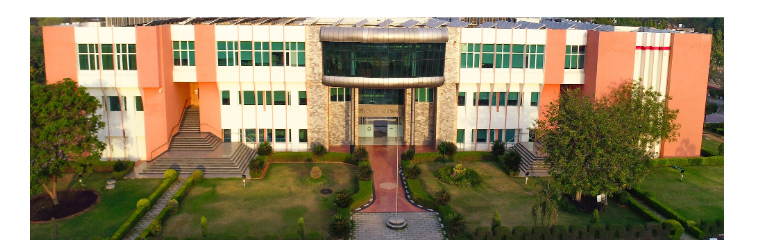
\includegraphics[width=\linewidth]{pic2.png}
    \caption{This is a floating image and can appear anywhere.}
    \label{fig:placeholder}
\end{minipage}
    
\end{figure}
\end{document}
